\section{Evaluations}
\label{sec:eval}
In this section, we evaluate the system with several experiments,
including the function, efficiency and overall test.
Furthermore, we conduct some more experiments to analyze the large number of
top-$k$ lists we extracted from the whole web,
from which we can find some interesting features of top-$k$ lists as well as pages.

There are two main working environment of these experiments.
For functional test, efficiency test and result analysis,
experiments are conducted in our local machine with 3GB RAM and 2.70GHz Dual-Core CPU.
For the big data experiment in the overall test, we deployed our system on \emph{Cosmos},
a large distributed system maintained by MSRA.

The top-$k$ list is a brand new subarea in web mining,
which is recently introduced\cite{ZZX2012KDD}
and rarely studied.
Although there were many previous attempts
\cite{googlesets,webtables08,LiuGZ03:MDR,MiaoTHSM09:TagPathClustering,GatterbauerBHKP2007:Towards,FumarolaWBMH11:List}
to extract general lists and tables from the web,
none of them targets on top-$k$ lists or solves this problem.
In addition we can hardly find implementation of these algorithms in the web.
Therefore, we cannot set up effective peer comparisons.
Instead, we compare it with our previous version\cite{ZZX2012KDD},
to show the the significant improvement of the current system.
%To highlight the improvement of the current system,
%we also compare it with the previous version of the system\cite{ZZX2012KDD}
%in some experiments.

%
%In this section, we conduct several experiments to evaluate the system.
%First we test each main functions separately with a specified benchmark.
%Then for the whole system, we evaluate its time efficiency and scalability.
%To test the actual performance in real massive web data, we deploy our system
%on a massive distributed computing platform to process the snapshot of all the web pages.
%Furthermore, we also conduct some experiments to analyze the large number of
%top-$k$ lists we extracted from the whole web,
%from which we can find some interesting features of top-$k$ lists as well as pages.


\subsection{Function Test}
\subsubsection{Title Recognition}
\label{sec:evalTitle}

%We test the performance of the CRF model in this subsection. We
To test the performance of the CRF model,
build a benchmark with 2000 random web page titles,
all of which contains at least one number.
50 of these are ``top-$k$ like'' and are treated as ground truth.

The classifier returns 60 titles, 46 of which are
true positives.
Therefore, the F-measure of the classifier is around 83.7\%
(Precision $\approx76.7\%$, Recall $=92\%$).
%Therefore, the precision of the classifier is
%$46/60\approx76.7\%$, while the recall is $46/50=92\%$ (F-measure$\approx83.7\%$).
The high recall ensures that most of the real top-$k$ pages can pass
through this stage.
%The 14 false positives are mostly due to misunderstanding of
%some regular phrases, such as ``six pixels of separation''
%and ``FIFA 10 cheat codes''.
%We can filter these errors in the following stages.

\subsubsection{Date and Location Detection}

%In this subsection we test the accuracy performance of date and location detection function.
%We build a benchmark with 1000 ``top-$k$ like'' titles.
We test the accuracy performance of date and location detection function,
using a benchmark of 1000 ``top-$k$ like'' titles.
By manually checking these titles,
we find 70 of them contain date information while 67 of them contain location information.
We consider these titles as ground truth.

We use the detector to process the benchmark, the result is shown in Table \ref{tab:whRes}.

\begin{table}
\centering
\caption{Results for Date and Location Detection}
\begin{tabular}{|c||c|c|c|}
\hline
Type  & Precision & Recall &  F-measure \\\hline
Date  & 83.5\% & 94.3\% & 88.6\%\\
Location & 87.3\% & 82.1\% & 84.6\%\\
\hline
\end{tabular}

\label{tab:whRes}
\end{table}

\subsubsection{List Extraction}

\label{sec:evalList}

Since HTML Parser, Candidate Picker and Top-K Ranker all serve for list extraction,
we put the three components together as one function and test the accuracy performance.
%We test accuracy performance of the system's list extractor,
%including HTML Parser, Candidate Picker and Top-K Ranker.
We set up a benchmark of 200 correct top-$k$ web pages,
all of which are readonly selected from the web.

%In order to compare the current algo with previous ones,
%we uses the list extractor to process the same benchmark,
%which consists of 100 correct top-$k$ pages.

The result is shown in Table \ref{tab:listRes}.
In this table, we also list the result for the two algorithms of the original system\cite{ZZX2012KDD}.
We can see that, the current system has the highest F-measure among the three versions.
Especially, it gains a very high precision.
%and it is better than the original one in both precision and recall.
Later we will see the advantage of current system is even larger for big data.

\begin{table}
\centering
\caption{Results for List Extraction}
\begin{tabular}{|c||c|c|c|}
\hline
Algo  & Precision & Recall & F-measure\\\hline
Default  & 89.3\% & 83.5\% & 86.3\% \\
Def+Patt  & 95.4\% & 72.0\% & 82.1\% \\
Current  & \textbf{97.5\%} & \textbf{78.0\%} & \textbf{86.7\%}\\
\hline
\end{tabular}

\label{tab:listRes}
\end{table}

\subsection{Time Efficiency Test}

We also record the running time for each step to test efficiency.
In average, the system takes 128 ms to process one top-$k$ page,
most of which is consumed by the HTML parser (77 ms). The main algorithm,
including Candidate Picker, Top-K Ranker and Content Processor,
only takes up about 1/3 of total running time (40 ms).

In addition, if Title Classifier recognizes a page not a top-$k$ page,
the system directly returns without processing the page content.
Therefore, for these ``non-top-$k$'' pages, it only costs the time for Title Classifier,
which is 9 ms in average.


%We also record the average running time for each step to test efficiency,
%which is listed in Table \ref{tab:TimeCostDistribution}.
%In this table, \emph{Algo} means the time cost by the main algorithm,
%including Candidate Picker Top-K Ranker and Content Processor.
%While \emph{Parse} is for HTML parser,
%%``Probase'' is the time cost in Probase Connector,
%and \emph{Title} is for Title Classifier.
%
%The data shows high efficiency of our system,
%the algorithm only takes up about 1/4 of total running time.
%
%\begin{table}[tb]
%\centering
%\caption{Average Execution Time of Different Stages (Unit:ms)}
%\label{tab:TimeCostDistribution}
%\begin{tabular}{|c||c|c|c|}
%\hline
%%\textbf{Total} & Algo & Parse & Title \\\hline
%%128 & 33 & 77 & 9\\\hline
%
%\textbf{Total} & Algo & Parse & Title \\\hline
%128 & 40 & 77 & 9\\\hline
%
%\end{tabular}
%\end{table}

Also, we conduct a scaling test of file size,
which is shown in Figure \ref{fig:FileSize}.
The test set consists of 300 "top-$k$" pages with proper size.
The result shows a certain positive correlation between file size and running time.

\begin{figure*}[th]
\centering
\subfigure[Scaling Test of File Size]{
  \label{fig:FileSize}
  \epsfig{file=./pics/filesize.eps,width=0.47\columnwidth}
}
\subfigure[The Performance for Big Data]{
  \label{fig:big}
  \epsfig{file=./pics/bigdata.eps,width=0.47\columnwidth}
}
\subfigure[The Distribution of Number K]{
  \label{fig:kDistri}
  \epsfig{file=./pics/k_distribute.eps,width=0.47\columnwidth}
}
\subfigure[The Distribution of Column Number]{
  \label{fig:colDistri}
  \epsfig{file=./pics/col_distribute.eps,width=0.47\columnwidth}
}
\caption{Experimental Results}
\label{fig:results}
\end{figure*}


%\begin{figure}[th]
%	\centering
%	\epsfig{file=./pics/filesize.eps,width=0.9\columnwidth}
%	\caption{Scaling Test of File Size}
%	\label{fig:FileSize}
%\end{figure}

\subsection{Overall Test}

\subsubsection{The Sum of Top-K Pages }
\label{sec:topKSum}
%
%In our demo paper, we have estimated the sum of top-$k$ pages.
%We sampled 1000 normal web pages and find 14 top-$k$ pages.
%Thus the total number should be $1.4\textperthousand \times 1,600,000,000 \approx 2,240,000$
%(assuming that there are 1.6 billion web pages in total).

As we need to calculate the recall for the overall system,
we must estimate the total number of top-$k$ pages.
Known that the recall of the title classifier is 92\%,
we use it to identify 1.6 million pages
(about 1/1000 of total pages in the web), and obtain 5994 pages.
By manually check these pages,
we find 2,061 of them are real top-$k$ pages.
Considering there are 8\% missed by the classifier,
the total number of top-$k$ pages should be $2,061\div92\%\approx2,240$.
Therefore the total number of top-$k$ pages should be approximately $2,240\times1,000=2,240,000$.
Assuming that there are 1.6 billion web pages in total, the proportion of top-$k$ pages are $2,240,000 \div 1,600,000,000\approx0.0014=1.4$\textperthousand.

\subsubsection{Big Data Experiment}
\label{eval:bigdata}
%One of the purpose for our system is to extract the
%``top-$k$ lists'' from the whole web.
We want to test the system's overall performance for real web pages,
and extract as many top-$k$ lists as possible from the whole Internet.
Therefore, we apply the framework on the high-frequency web snapshot from Bing,
which are about 1.6 billion.
Our system finally extracted 1,753,124 top-$k$ lists.
By sampling analysis, we find the precision is 92\%,
which means that there should be about 1,612,874 true positives.
According to the estimated sum of top-$k$ pages,
the recall should be $1,612,874\div2,240,000\approx72.0\%$.

Before this paper, we implemented a prototype system
and processed a smaller page set (1/10 of the web)\cite{ZZX2012KDD}.
To compare their accuracy performance, we put these result together,
which is shown in Figure \ref{fig:big}.
Among the three systems,
the current system obtains the highest F-measure (about 80.8\%).
Since {\em Default} is not very useful due to its low precision (66\%),
we mainly compare the current algorithm with {\em Def+Patt}.
It is apparent that the current is better in both Precision and Recall.
Especially, the current system shows significant improvement in the recall,
which make it extracted about 400,000 more lists than expect from the whole web.

%\begin{figure}[th]
%	\centering
%	\epsfig{file=./pics/bigdata.eps,width=0.9\columnwidth}
%\caption{The Performance for Big Data}
%\label{fig:big}
%\end{figure}

%Since the work of the system is independent,
%the system is easy to run on multiple machines concurrently.
%In this experiment, we apply the system to a distributive computing system to extract data
%To analyze the precision of both algorithm, we randomly sample 100 lists from each result data.
%According to the estimated sum of top-$k$ pages,
%there should be in total 224,000 top-$k$ pages (ground truth)
%in the input data. The detailed result is shown in Table \ref{tab:cosmosRes}.
%
%\begin{table}
%\centering
%\begin{tabular}{|c||c|c|c|c|}
%\hline
%Algo & Total & Precision & True Positive & Recall\\\hline
%Default & 256,231 & 66.0\% & 169,112 & 75.5\% \\
%Def+Patt& 142,886 & 90.4\% & 129,169 & 57.7\% \\
%\hline
%\end{tabular}
%\caption{Results for Big Data}
%\label{tab:cosmosRes}
%\vspace*{-10pt}
%\end{table}
%
%From Table \ref{tab:cosmosRes}, we can see that {\em Def+Patt}
%obtains over 90\% precision,
%while the recall is lower than {\em Default}. Nevertheless,
%{\em Def+Patt} still manage to obtain a large number of top-$k$ lists.
%If we project up to the whole web snapshot,
%{\em Def+Patt} is expected to get over 1.4 million
%``top-$k$ list'' with over 90\% precision.

\subsection{Result Analysis}
With the result data we obtained from the experiments above,
we do some analysis and find some interesting features about top-$k$ lists.
In the following two experiments,
we use 100,000 of the result top-$k$ list (about 1/15 of all lists)  as sample test set.

\subsubsection{K Distribution}
The first experiment is to study the distribution of the number $k$.
As is limited by the system, a proper $k$ should be larger than 2 and smaller than 5000.
In our sample set, the largest $k$ equals to 4,526.
Figure \ref{fig:kDistri} shows the distribution for $k\leq35$.
From this figure,
multiples of 5 and 10 are more popular than their neighbors.
Especially, 5 and 10 are the two most  popular number. They take up 65\% of all cases.
For rest numbers, the count is decreasing in the rough as the $k$ grows.

The experimental result is consistent with our common sense.
The editors of top-$k$ pages prefer to use a multiple of 5 or 10 as $k$,
since it is easier to remember.
And generally they may not choose a too large number
since it is difficult to place all list items into a single page.

%\begin{figure}[th]
%	\centering
%	\epsfig{file=./pics/k_distribute.eps,width=\columnwidth}
%\caption{The Distribution of Number K}
%\label{fig:kDistri}
%\end{figure}

\subsubsection{Column Number Distribution}
We also draw a distribution graph for column number($\leq20$), which is Figure \ref{fig:colDistri}.
In this sample set, the largest column number is 62.
Figure \ref{fig:colDistri}, we can know the most (80\%) of the lists contain no more than 3 columns.
And for rest lists, the count is is decreasing in the rough as the column number grows.


%\begin{figure}[th]
%	\centering
%	\epsfig{file=./pics/col_distribute.eps,width=\columnwidth}
%\caption{The Distribution of Column Number}
%\label{fig:colDistri}
%\end{figure}
